% A LaTeX (non-official) template for ISAE projects reports
% Copyright (C) 2014 Damien Roque
% Version: 0.2
% Author: Damien Roque <damien.roque_AT_isae.fr>

% Updated version for Ensimag homework reports by Yoan Souty

\documentclass[a4paper,12pt, openany, twoside]{article}
\usepackage[utf8]{inputenc}
\usepackage[T1]{fontenc}
\usepackage[frenchb]{babel} % If you write in French
%\usepackage[english]{babel} % If you write in English
\usepackage{a4wide}
\usepackage{lipsum}
\usepackage{graphicx}
\graphicspath{{images/}} % emplacement des images
\usepackage{subfig}
 \usepackage{float}
\usepackage{tikz}
\usetikzlibrary{shapes,arrows}
\usepackage{pgfplots}
\pgfplotsset{compat=newest}
\pgfplotsset{plot coordinates/math parser=false}
\newlength\figureheight
\newlength\figurewidth
\pgfkeys{/pgf/number format/.cd,
set decimal separator={,\!},
1000 sep={\,},
}
\usepackage{ifthen}
\usepackage{ifpdf}
\ifpdf
\usepackage[pdftex]{hyperref}
\else
\usepackage{hyperref}
\fi
\usepackage{color}
\hypersetup{%
colorlinks=true,
linkcolor=black,
citecolor=black,
urlcolor=black}

\usepackage{titlesec}
\titleformat{\section}[hang]{\bf\huge}{\thesection}{2pc}{}

\renewcommand{\thesection}{\Roman{section}}


\renewcommand{\baselinestretch}{1.05}
\usepackage{fancyhdr}
\pagestyle{fancy}
\renewcommand{\sectionmark}[1]{\markboth{\thesection .\ #1}{}}
\renewcommand{\subsectionmark}[1]{\markright{\thesubsection .\ #1}}
\fancyhead{}
\fancyhead[RE]{\nouppercase{\leftmark}}
\fancyhead[LO]{\nouppercase{\rightmark}}
\renewcommand{\headrulewidth}{0pt}

\let\headruleORIG\headrule
\renewcommand{\headrule}{\color{black} \headruleORIG}
\renewcommand{\headrulewidth}{1.0pt}
\usepackage{colortbl}
\arrayrulecolor{black}

\fancypagestyle{plain}{
  \fancyhead{}
  \fancyfoot[C]{\thepage}
  \renewcommand{\headrulewidth}{0pt}
}

\makeatletter
\def\@textbottom{\vskip \z@ \@plus 1pt}
\let\@texttop\relax
\makeatother

\makeatletter
\def\cleardoublepage{\clearpage\if@twoside \ifodd\c@page\else%
  \hbox{}%
  \thispagestyle{empty}%
  \newpage%
  \if@twocolumn\hbox{}\newpage\fi\fi\fi}
\makeatother

\usepackage{amsthm}
\usepackage{amssymb,amsmath,bbm}
\usepackage{array}
\usepackage{bm}
\usepackage{multirow}
\usepackage[footnote]{acronym}
\usepackage{mathtools}

\DeclarePairedDelimiter\ceil{\lceil}{\rceil}
\DeclarePairedDelimiter\floor{\lfloor}{\rfloor}

\newcommand*{\SET}[1]  {\ensuremath{\mathbf{#1}}}
\newcommand*{\VEC}[1]  {\ensuremath{\boldsymbol{#1}}}
\newcommand*{\FAM}[1]  {\ensuremath{\boldsymbol{#1}}}
\newcommand*{\MAT}[1]  {\ensuremath{\boldsymbol{#1}}}
\newcommand*{\OP}[1]  {\ensuremath{\mathrm{#1}}}
\newcommand*{\NORM}[1]  {\ensuremath{\left\|#1\right\|}}
\newcommand*{\DPR}[2]  {\ensuremath{\left \langle #1,#2 \right \rangle}}
\newcommand*{\calbf}[1]  {\ensuremath{\boldsymbol{\mathcal{#1}}}}
\newcommand*{\shift}[1]  {\ensuremath{\boldsymbol{#1}}}

\newcommand{\eqdef}{\stackrel{\mathrm{def}}{=}}
\newcommand{\argmax}{\operatornamewithlimits{argmax}}
\newcommand{\argmin}{\operatornamewithlimits{argmin}}
\newcommand{\ud}{\, \mathrm{d}}
\newcommand{\vect}{\text{Vect}}
\newcommand{\sinc}{\ensuremath{\mathrm{sinc}}}
\newcommand{\esp}{\ensuremath{\mathbb{E}}}
\newcommand{\hilbert}{\ensuremath{\mathcal{H}}}
\newcommand{\fourier}{\ensuremath{\mathcal{F}}}
\newcommand{\sgn}{\text{sgn}}
\newcommand{\intTT}{\int_{-T}^{T}}
\newcommand{\intT}{\int_{-\frac{T}{2}}^{\frac{T}{2}}}
\newcommand{\intinf}{\int_{-\infty}^{+\infty}}
\newcommand{\Sh}{\ensuremath{\boldsymbol{S}}}
\newcommand{\C}{\SET{C}}
\newcommand{\R}{\SET{R}}
\newcommand{\Z}{\SET{Z}}
\newcommand{\N}{\SET{N}}
\newcommand{\K}{\SET{K}}
\newcommand{\reel}{\mathcal{R}}
\newcommand{\imag}{\mathcal{I}}
\newcommand{\cmnr}{c_{m,n}^\reel}
\newcommand{\cmni}{c_{m,n}^\imag}
\newcommand{\cnr}{c_{n}^\reel}
\newcommand{\cni}{c_{n}^\imag}
\newcommand{\tproto}{g}
\newcommand{\rproto}{\check{g}}
\newcommand{\LR}{\mathcal{L}_2(\SET{R})}
\newcommand{\LZ}{\ell_2(\SET{Z})}
\newcommand{\LZI}[1]{\ell_2(\SET{#1})}
\newcommand{\LZZ}{\ell_2(\SET{Z}^2)}
\newcommand{\diag}{\operatorname{diag}}
\newcommand{\noise}{z}
\newcommand{\Noise}{Z}
\newcommand{\filtnoise}{\zeta}
\newcommand{\tp}{g}
\newcommand{\rp}{\check{g}}
\newcommand{\TP}{G}
\newcommand{\RP}{\check{G}}
\newcommand{\dmin}{d_{\mathrm{min}}}
\newcommand{\Dmin}{D_{\mathrm{min}}}
\newcommand{\Image}{\ensuremath{\text{Im}}}
\newcommand{\Span}{\ensuremath{\text{Span}}}

\newtheoremstyle{break}
  {11pt}{11pt}%
  {\itshape}{}%
  {\bfseries}{}%
  {\newline}{}%
\theoremstyle{break}

%\theoremstyle{definition}
\newtheorem{definition}{Définition}[section]

%\theoremstyle{definition}
\newtheorem{theoreme}{Théorème}[section]

%\theoremstyle{remark}
\newtheorem{remarque}{Remarque}[]

%\theoremstyle{plain}
\newtheorem{propriete}{Propriété}[section]
\newtheorem{exemple}{Exemple}[section]

\newtheorem{question}{Question}[section]

\parskip=5pt
%\sloppy

\begin{document}

%%%%%%%%%%%%%%%%%%
%%% First page %%%
%%%%%%%%%%%%%%%%%%

\begin{titlepage}
\begin{center}


\includegraphics[width=0.6\textwidth]{ensimag_logo.png}\\[1cm]

{\large Ensimag MMIS 3A}\\[0.5cm]

{\large Ondelettes et applications à l'image}\\[0.5cm]

% Title
\rule{\linewidth}{0.5mm} \\[0.4cm]
{ \huge \bfseries Compte-rendu du lab2, part2\\[0.4cm] }
\rule{\linewidth}{0.5mm} \\[1.5cm]

% Author and supervisor
\noindent
\begin{minipage}{0.4\textwidth}
  \begin{flushleft} \large
    \emph{Auteurs :}\\
    % M\up{me} Prénom \textsc{Nom}\\
    M. Antonin \textsc{Klopp-Tosser}\\
    M. Yoan \textsc{Souty} \\
  \end{flushleft}
\end{minipage}%
\begin{minipage}{0.4\textwidth}
  \begin{flushright} \large
    \emph{Encadrante :} \\
    M\up{me} Valérie \textsc{Perrier} \\

    % Dr.~Prénom \textsc{Nom}
  \end{flushright}
\end{minipage}

\vfill

% Bottom of the page
{\large \today}

\end{center}
\end{titlepage}

%%%%%%%%%%%%%%%%%%%%%%%%%%%%%
%%% Non-significant pages %%%
%%%%%%%%%%%%%%%%%%%%%%%%%%%%%


%%%%%%%%%%%%%%%%%%%%%%%%%%%%%%%%%%%%%%%%%%%%
%%% Content of the report and references %%%
%%%%%%%%%%%%%%%%%%%%%%%%%%%%%%%%%%%%%%%%%%%%

\pagestyle{fancy}


\tableofcontents

\clearpage

\listoffigures

\clearpage

\section{Compression d'images 2D}
La compression a été testée sur plusieurs images générées à partir de la fonction \texttt{ReadImage}. Nous avons utilisé la famille orthogonale \textit{Daubechies}, avec un \textit{vanishing moment} de 4. Le taux de compression $\tau$ est donné en paramètre dans le script, le calcul du nombre de coefficients $N_{comp}$ à conserver se déduit donc avec la formule suivante :

  $N_{comp} = \floor* {N_{total} * (1 - \tau)}$

Nous avons cependant constaté que la compression n'était affectée que pour un taux de compression $\tau$ anormalement très élevé (e.g $\tau \approx 0.9999$).


% \begin{figure}[H]
%   
\includegraphics[width=0.4\textwidth]{ensimag_logo}\hfill
%   
\includegraphics[width=0.4\textwidth]{ensimag_logo}
%   \subfloat[\label{fig:ref1} une légende]{\hspace{.5\linewidth}}
%   \subfloat[\label{fig:ref2} une autre]{\hspace{.5\linewidth}}
%   \caption{légende globale}
%   \label{fig:ref}
% \end{figure}
\begin{figure}[H]
  \centering
  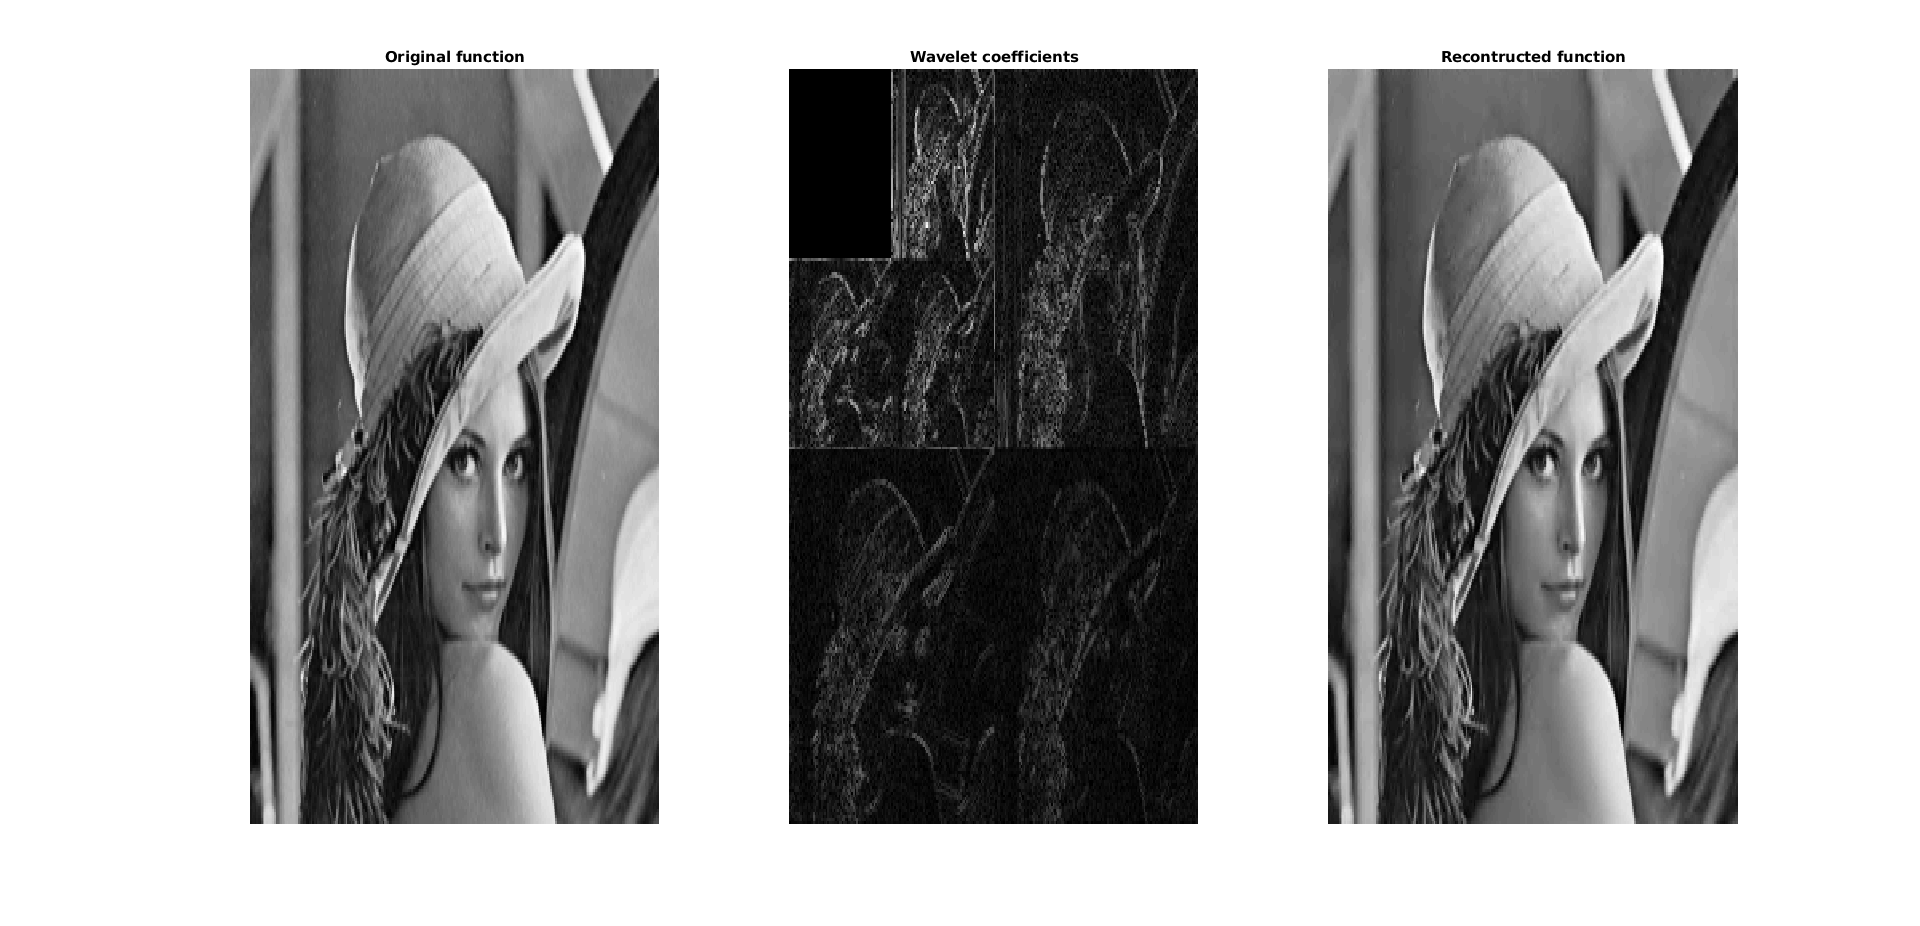
\includegraphics[width=0.75\textwidth]{comp_lenna}\vfill
  \caption{Compression avec $\tau=0.75$}
\end{figure}

\begin{figure}[H]
  \centering
  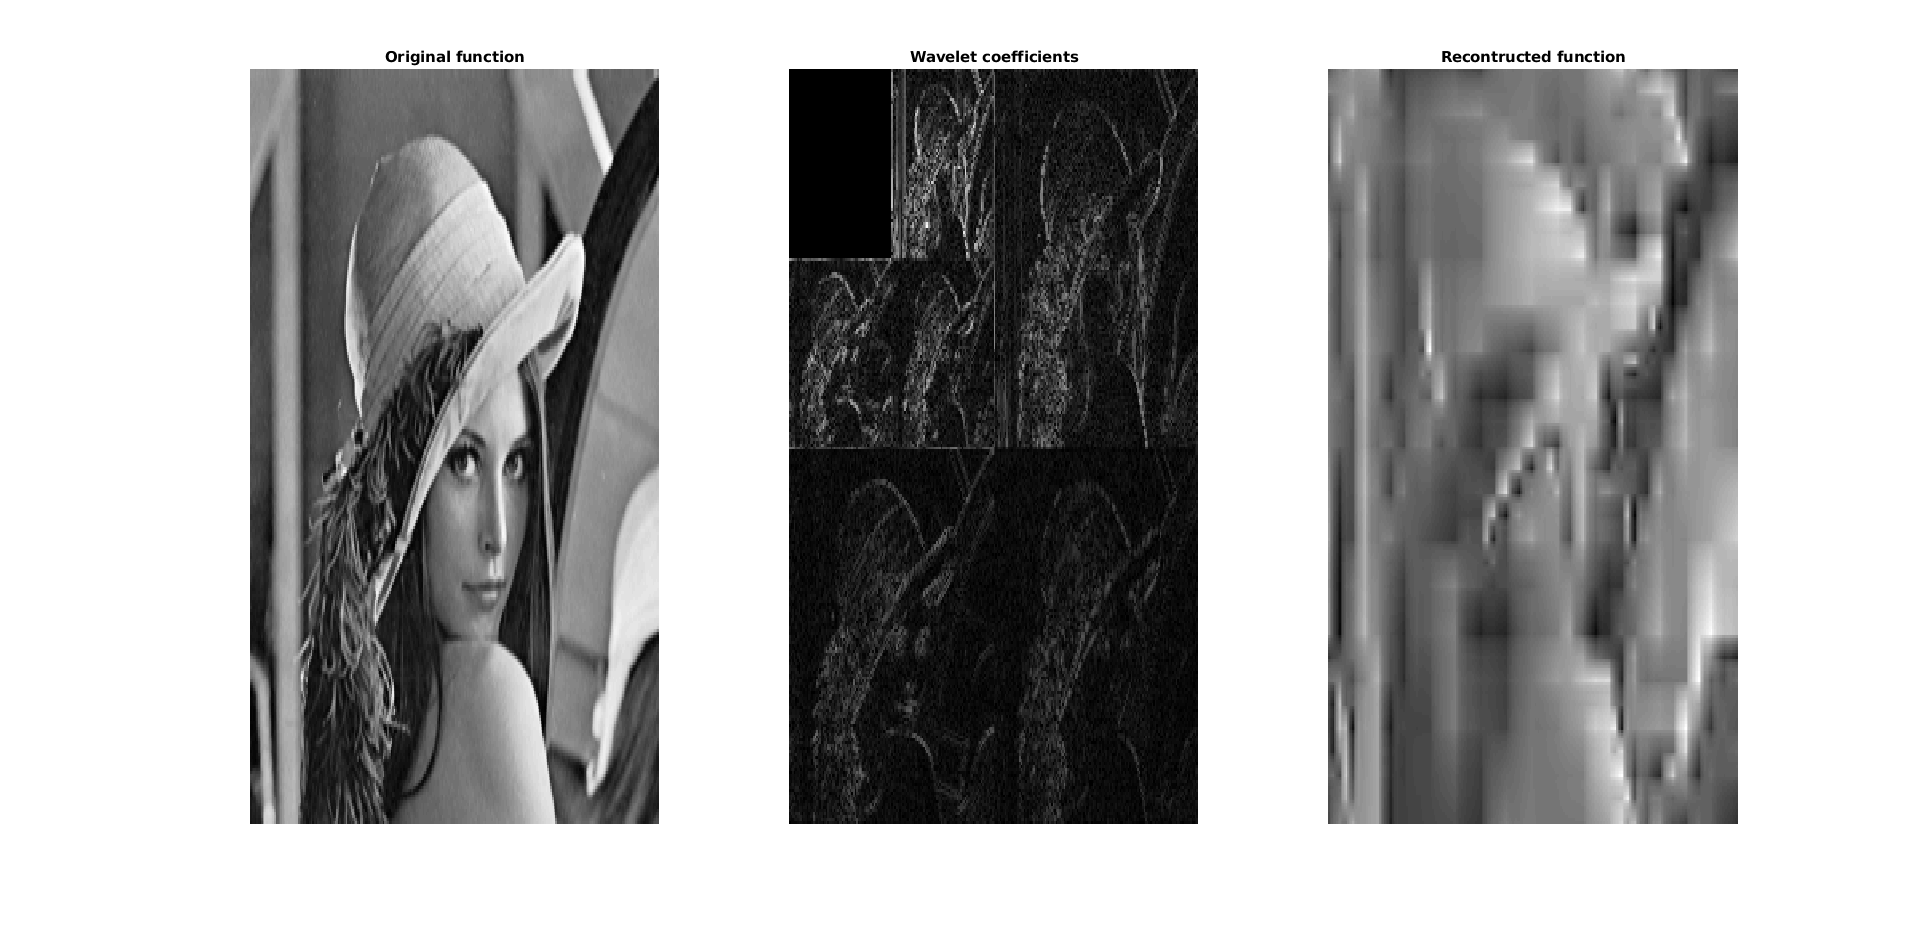
\includegraphics[width=0.75\textwidth]{comp_lenna2}\vfill
  \caption{Compression avec $\tau=0.9999$}
\end{figure}


\section{Débruitages d'images}
On considère une image 2D, bruitée par un signal Gaussien de moyenne nulle, d'écart-type $\sigma > 0$. On utilise la fonction \texttt{ThreshWave2} qui prend en argument le signal bruité (de longueur de la forme $2^J$), le filtre miroir en quadrature (\texttt{qmf}), et calcule le signal estimé. La fonction estime automatiquement $\sigma$ à l'aide de la valeur médiane et permet d'opter au choix pour un \textit{soft thresholding} ou \textit{hard thresholding}.

La fonction \texttt{IdealWavDenoise} permet, à partir du signal original 1D, du signal bruité, du filtre quadrature miroir et de l'écart-type du bruit $\sigma$ de récupérer le signal estimé, ainsi que les coefficients d'ondelettes du signal bruité et du signal estimé. Par défaut, la fonction utilise la famille Symmlet, avec un \textit{vanishing moment} de 8.

\begin{figure}[!htp]
  \centering
  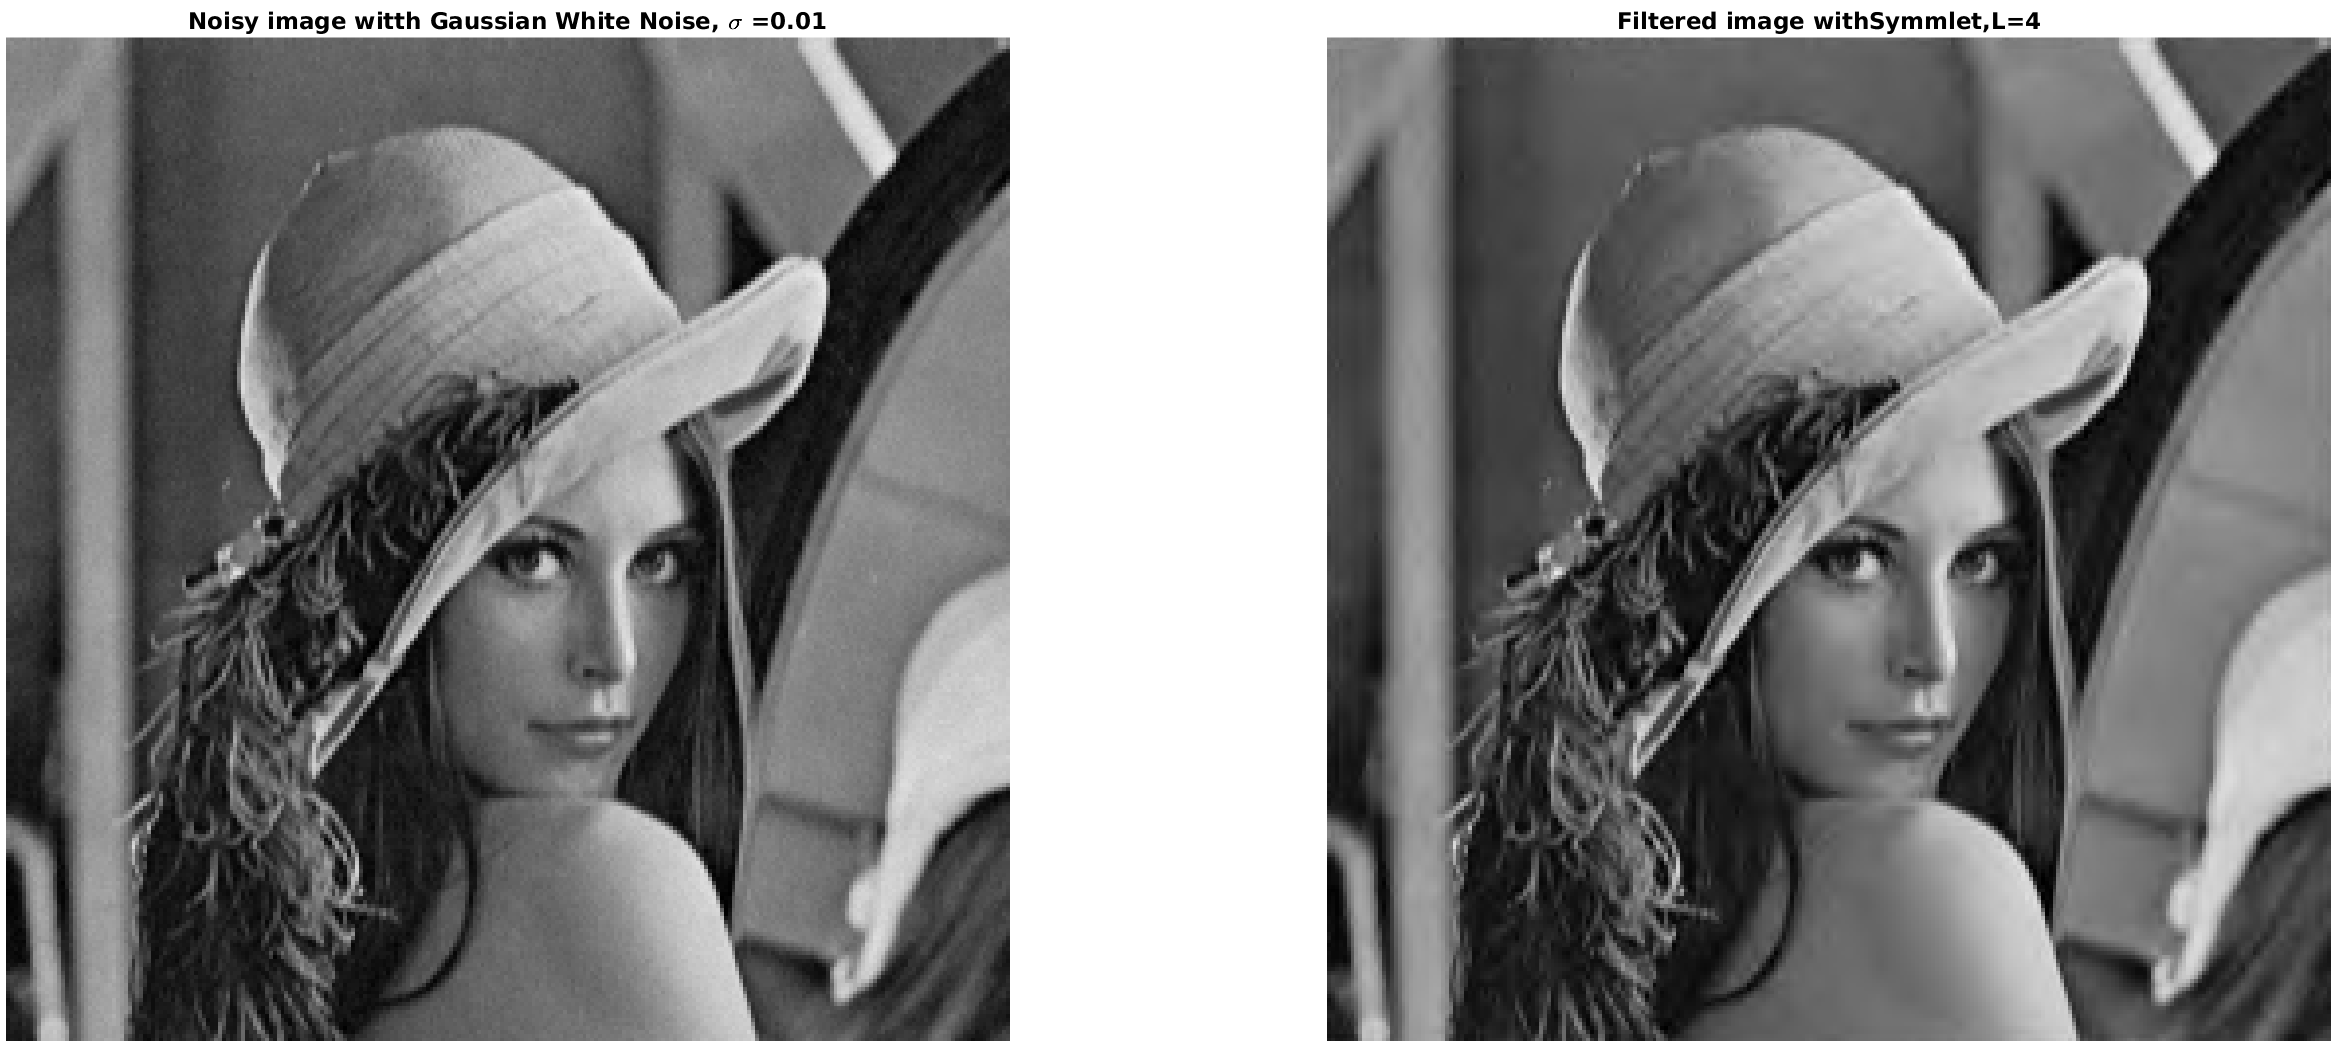
\includegraphics[width=0.75\textwidth]{denoise_lenna1}\vfill
  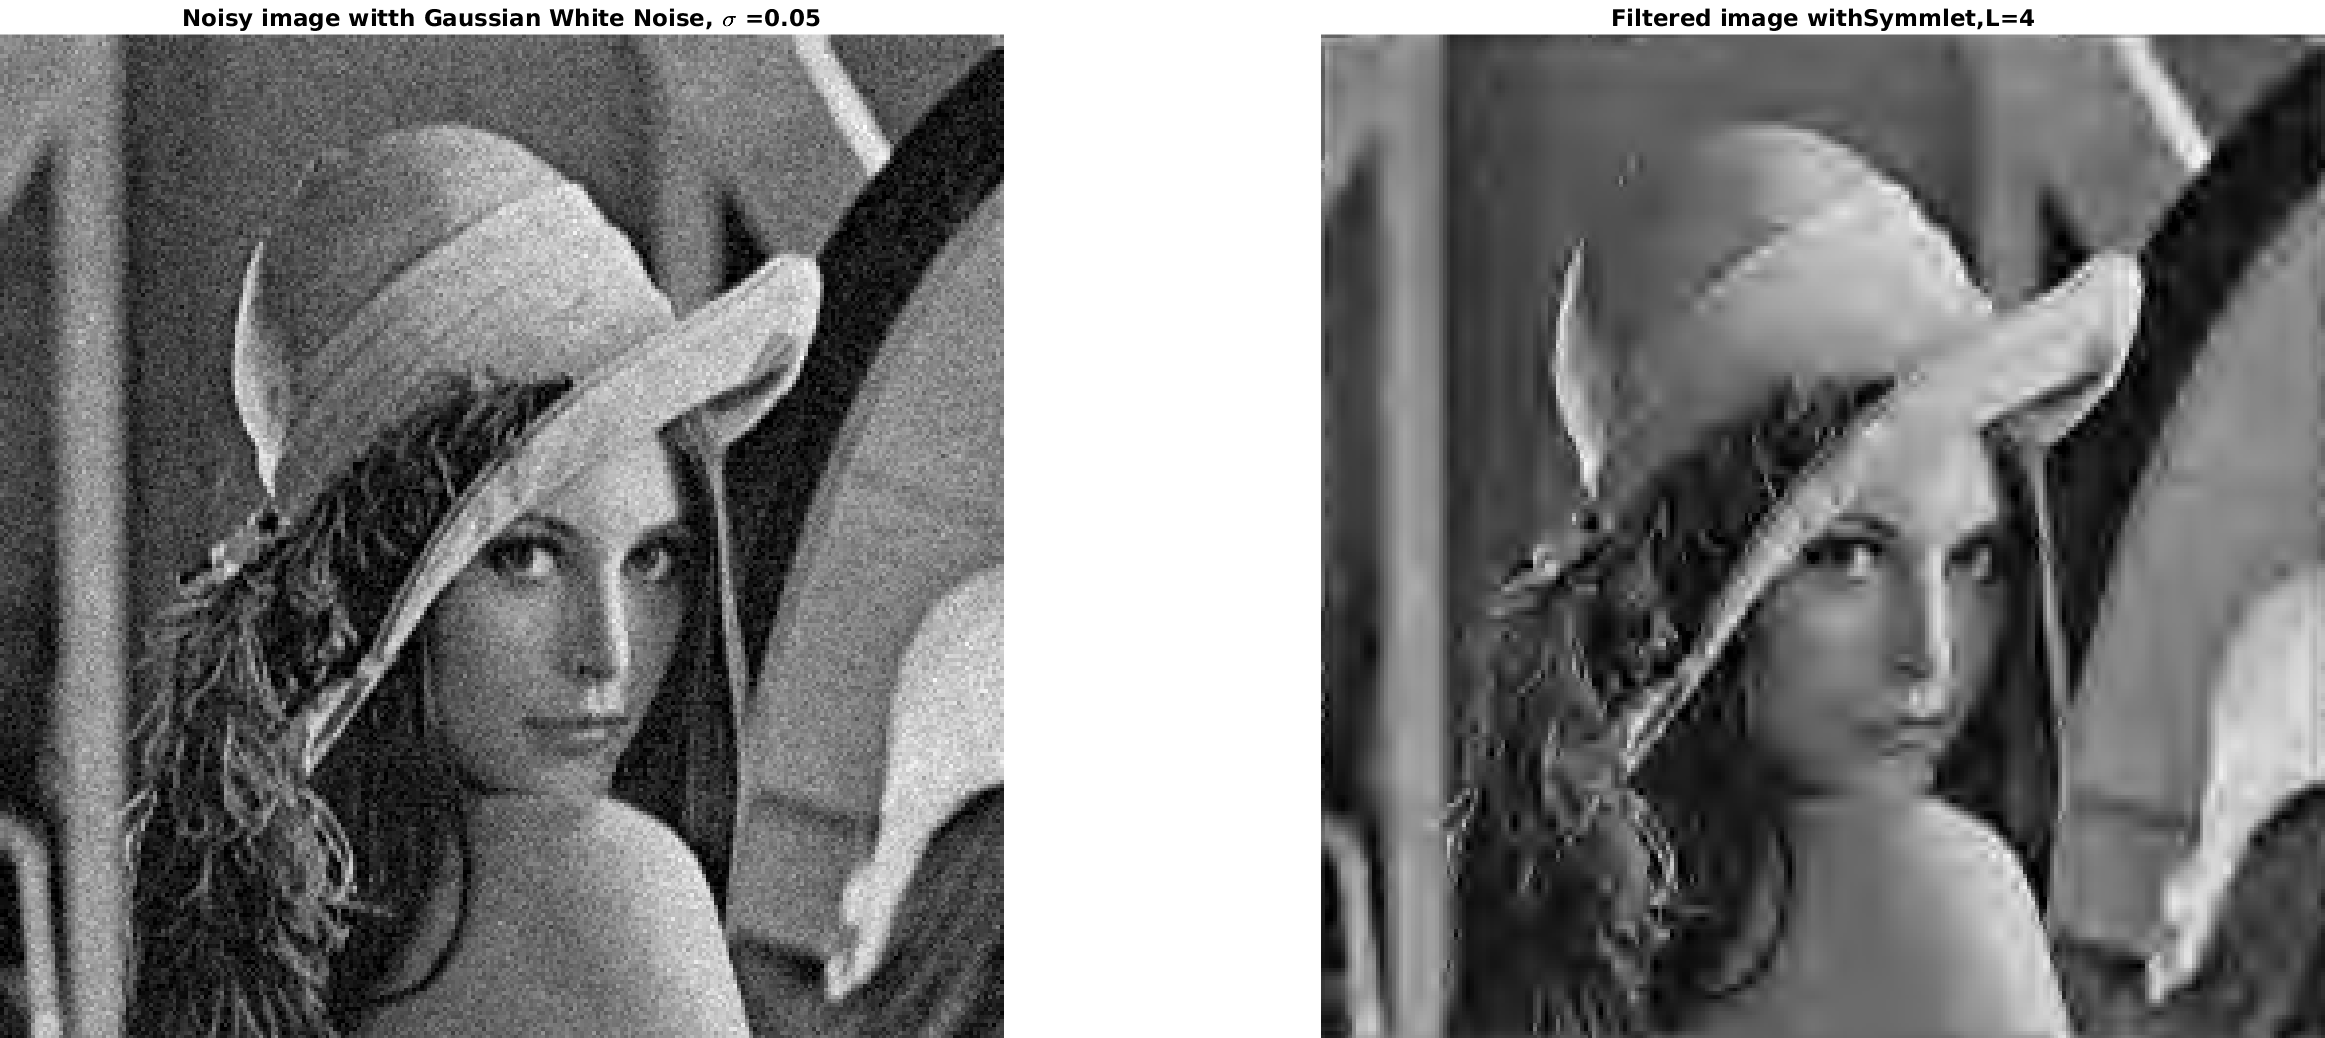
\includegraphics[width=0.75\textwidth]{denoise_lenna5}\vfill
  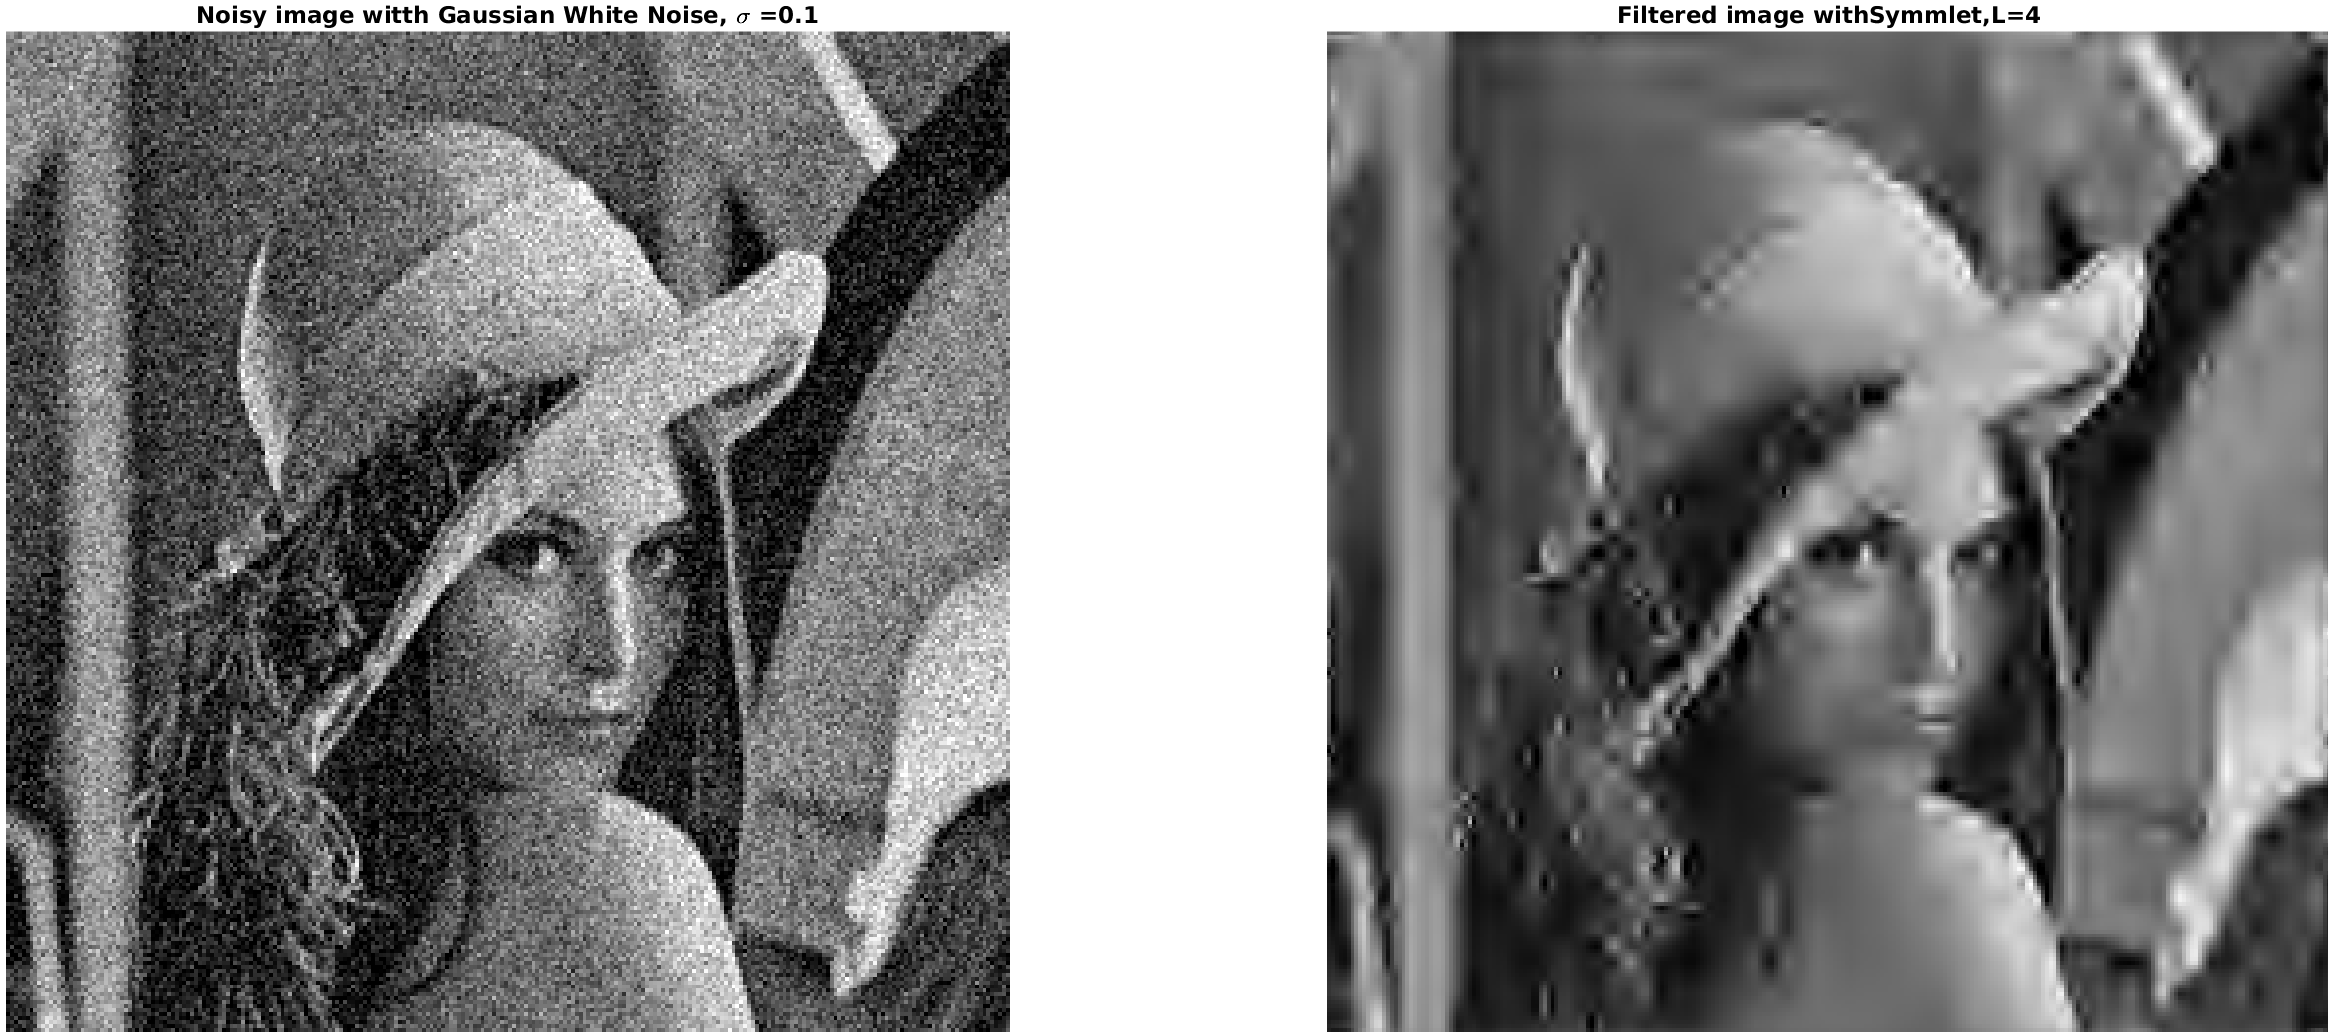
\includegraphics[width=0.75\textwidth]{denoise_lenna10}\vfill
  \caption{(De haut en bas) débruitage de Lenna avec $\sigma=0.01, 0.05, 0.1$}
\end{figure}




\end{document}
